\documentclass{standalone}
\usepackage{tikz}
\usetikzlibrary{patterns, positioning}


\begin{document}
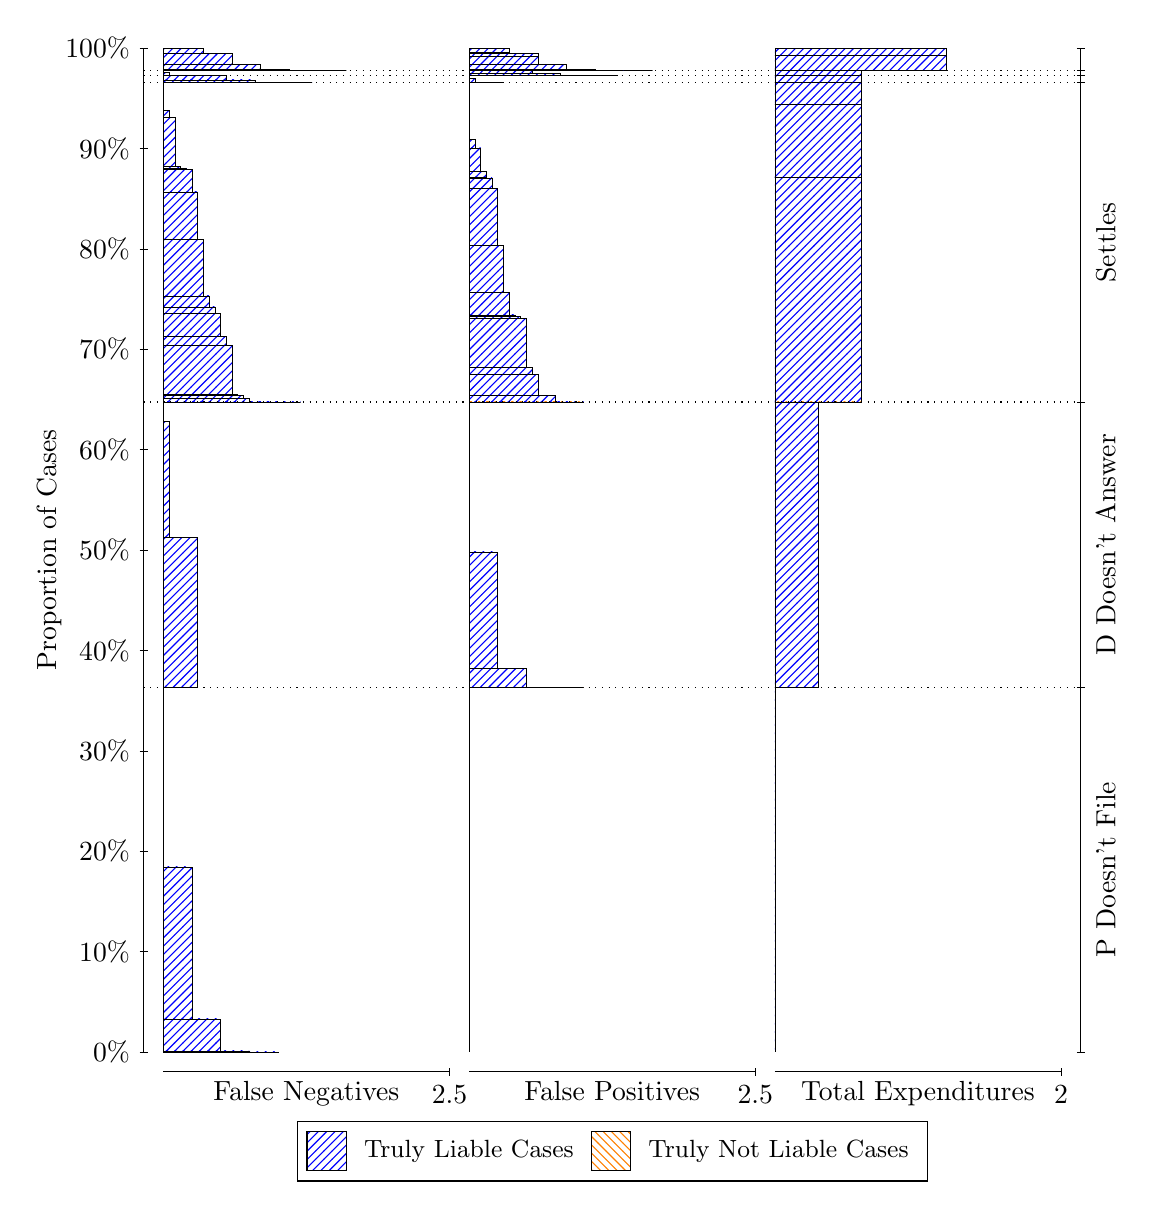
\begin{tikzpicture}
\draw[black, very thin] (1.5,1.75) -- (1.5,14.5);
\node[rotate=90, text=black, anchor=center] at (0.3, 8.125) {Proportion of Cases};
\draw[black, very thin] (1.45,1.75) -- (1.55,1.75);
\node[text=black, anchor=east] at (1.45, 1.75) {0\%};
\draw[black, very thin] (1.45,3.025) -- (1.55,3.025);
\node[text=black, anchor=east] at (1.45, 3.025) {10\%};
\draw[black, very thin] (1.45,4.3) -- (1.55,4.3);
\node[text=black, anchor=east] at (1.45, 4.3) {20\%};
\draw[black, very thin] (1.45,5.575) -- (1.55,5.575);
\node[text=black, anchor=east] at (1.45, 5.575) {30\%};
\draw[black, very thin] (1.45,6.85) -- (1.55,6.85);
\node[text=black, anchor=east] at (1.45, 6.85) {40\%};
\draw[black, very thin] (1.45,8.125) -- (1.55,8.125);
\node[text=black, anchor=east] at (1.45, 8.125) {50\%};
\draw[black, very thin] (1.45,9.4) -- (1.55,9.4);
\node[text=black, anchor=east] at (1.45, 9.4) {60\%};
\draw[black, very thin] (1.45,10.675) -- (1.55,10.675);
\node[text=black, anchor=east] at (1.45, 10.675) {70\%};
\draw[black, very thin] (1.45,11.95) -- (1.55,11.95);
\node[text=black, anchor=east] at (1.45, 11.95) {80\%};
\draw[black, very thin] (1.45,13.225) -- (1.55,13.225);
\node[text=black, anchor=east] at (1.45, 13.225) {90\%};
\draw[black, very thin] (1.45,14.5) -- (1.55,14.5);
\node[text=black, anchor=east] at (1.45, 14.5) {100\%};

\draw[black, very thin] (13.4,1.75) -- (13.4,14.5);
\draw[black, very thin] (13.35,1.75) -- (13.45,1.75);
\node[anchor=west] at (13.35, 1.75) {};
\draw[black, very thin] (13.35,6.3778) -- (13.45,6.3778);
\node[anchor=west] at (13.35, 6.3778) {};
\draw[black, very thin] (13.35,10.005) -- (13.45,10.005);
\node[anchor=west] at (13.35, 10.005) {};
\draw[black, very thin] (13.35,14.059) -- (13.45,14.059);
\node[anchor=west] at (13.35, 14.059) {};
\draw[black, very thin] (13.35,14.155) -- (13.45,14.155);
\node[anchor=west] at (13.35, 14.155) {};
\draw[black, very thin] (13.35,14.219) -- (13.45,14.219);
\node[anchor=west] at (13.35, 14.219) {};
\draw[black, very thin] (13.35,14.5) -- (13.45,14.5);
\node[anchor=west] at (13.35, 14.5) {};

\draw[black, very thin, pattern color=blue, pattern=north east lines] (1.75,1.75) rectangle (3.2033,1.7501);
\draw[black, very thin, pattern color=blue, pattern=north east lines] (1.75,1.7501) rectangle (2.84,1.7635);
\draw[black, very thin, pattern color=blue, pattern=north east lines] (1.75,1.7635) rectangle (2.4767,2.1703);
\draw[black, very thin, pattern color=blue, pattern=north east lines] (1.75,2.1703) rectangle (2.1133,4.0998);
\draw[black, very thin, pattern color=orange, pattern=north west lines] (1.75,4.0998) rectangle (1.75,4.0998);
\draw[black, very thin, pattern color=blue, pattern=north east lines] (1.75,4.0998) rectangle (1.75,6.3778);
\draw[black, very thin, pattern color=blue, pattern=north east lines] (1.75,6.3778) rectangle (2.186,8.2833);
\draw[black, very thin, pattern color=blue, pattern=north east lines] (1.75,8.2833) rectangle (1.8227,9.7612);
\draw[black, very thin, pattern color=orange, pattern=north west lines] (1.75,9.7612) rectangle (1.75,9.7612);
\draw[black, very thin, pattern color=blue, pattern=north east lines] (1.75,9.7612) rectangle (1.75,10.005);
\draw[black, very thin, pattern color=blue, pattern=north east lines] (1.75,10.005) rectangle (3.494,10.005);
\draw[black, very thin, pattern color=blue, pattern=north east lines] (1.75,10.005) rectangle (3.2033,10.006);
\draw[black, very thin, pattern color=blue, pattern=north east lines] (1.75,10.006) rectangle (3.1307,10.007);
\draw[black, very thin, pattern color=blue, pattern=north east lines] (1.75,10.007) rectangle (3.058,10.007);
\draw[black, very thin, pattern color=blue, pattern=north east lines] (1.75,10.007) rectangle (2.9127,10.007);
\draw[black, very thin, pattern color=blue, pattern=north east lines] (1.75,10.007) rectangle (2.84,10.046);
\draw[black, very thin, pattern color=blue, pattern=north east lines] (1.75,10.046) rectangle (2.7673,10.093);
\draw[black, very thin, pattern color=blue, pattern=north east lines] (1.75,10.093) rectangle (2.6947,10.099);
\draw[black, very thin, pattern color=blue, pattern=north east lines] (1.75,10.099) rectangle (2.622,10.724);
\draw[black, very thin, pattern color=blue, pattern=north east lines] (1.75,10.724) rectangle (2.5493,10.833);
\draw[black, very thin, pattern color=blue, pattern=north east lines] (1.75,10.833) rectangle (2.4767,11.133);
\draw[black, very thin, pattern color=blue, pattern=north east lines] (1.75,11.133) rectangle (2.404,11.202);
\draw[black, very thin, pattern color=blue, pattern=north east lines] (1.75,11.202) rectangle (2.404,11.212);
\draw[black, very thin, pattern color=blue, pattern=north east lines] (1.75,11.212) rectangle (2.3313,11.352);
\draw[black, very thin, pattern color=blue, pattern=north east lines] (1.75,11.352) rectangle (2.2587,12.072);
\draw[black, very thin, pattern color=blue, pattern=north east lines] (1.75,12.072) rectangle (2.186,12.672);
\draw[black, very thin, pattern color=blue, pattern=north east lines] (1.75,12.672) rectangle (2.1133,12.954);
\draw[black, very thin, pattern color=blue, pattern=north east lines] (1.75,12.954) rectangle (2.0407,12.971);
\draw[black, very thin, pattern color=blue, pattern=north east lines] (1.75,12.971) rectangle (2.0407,12.971);
\draw[black, very thin, pattern color=blue, pattern=north east lines] (1.75,12.971) rectangle (1.968,12.995);
\draw[black, very thin, pattern color=blue, pattern=north east lines] (1.75,12.995) rectangle (1.8953,13.622);
\draw[black, very thin, pattern color=blue, pattern=north east lines] (1.75,13.622) rectangle (1.8227,13.712);
\draw[black, very thin, pattern color=orange, pattern=north west lines] (1.75,13.712) rectangle (1.75,13.712);
\draw[black, very thin, pattern color=blue, pattern=north east lines] (1.75,13.712) rectangle (1.75,14.059);
\draw[black, very thin, pattern color=blue, pattern=north east lines] (1.75,14.059) rectangle (3.6393,14.059);
\draw[black, very thin, pattern color=blue, pattern=north east lines] (1.75,14.059) rectangle (3.276,14.059);
\draw[black, very thin, pattern color=blue, pattern=north east lines] (1.75,14.059) rectangle (2.9127,14.095);
\draw[black, very thin, pattern color=blue, pattern=north east lines] (1.75,14.095) rectangle (2.5493,14.154);
\draw[black, very thin, pattern color=blue, pattern=north east lines] (1.75,14.154) rectangle (2.186,14.155);
\draw[black, very thin, pattern color=orange, pattern=north west lines] (1.75,14.155) rectangle (1.75,14.155);
\draw[black, very thin, pattern color=blue, pattern=north east lines] (1.75,14.155) rectangle (2.186,14.156);
\draw[black, very thin, pattern color=blue, pattern=north east lines] (1.75,14.156) rectangle (1.8227,14.195);
\draw[black, very thin, pattern color=orange, pattern=north west lines] (1.75,14.195) rectangle (1.75,14.195);
\draw[black, very thin, pattern color=blue, pattern=north east lines] (1.75,14.195) rectangle (1.75,14.219);
\draw[black, very thin, pattern color=blue, pattern=north east lines] (1.75,14.219) rectangle (4.0753,14.219);
\draw[black, very thin, pattern color=blue, pattern=north east lines] (1.75,14.219) rectangle (3.712,14.219);
\draw[black, very thin, pattern color=blue, pattern=north east lines] (1.75,14.219) rectangle (3.3487,14.224);
\draw[black, very thin, pattern color=blue, pattern=north east lines] (1.75,14.224) rectangle (2.9853,14.289);
\draw[black, very thin, pattern color=blue, pattern=north east lines] (1.75,14.289) rectangle (2.622,14.43);
\draw[black, very thin, pattern color=blue, pattern=north east lines] (1.75,14.43) rectangle (2.2587,14.495);
\draw[black, very thin, pattern color=blue, pattern=north east lines] (1.75,14.495) rectangle (1.8953,14.5);
\draw[black, very thin, pattern color=orange, pattern=north west lines] (1.75,14.5) rectangle (1.75,14.5);
\draw[black, very thin, pattern color=blue, pattern=north east lines] (1.75,14.5) rectangle (1.75,14.5);
\draw[black, very thin, pattern color=orange, pattern=north west lines] (5.6333,1.75) rectangle (5.6333,1.75);
\draw[black, very thin, pattern color=blue, pattern=north east lines] (5.6333,1.75) rectangle (5.6333,6.3778);
\draw[black, very thin, pattern color=orange, pattern=north west lines] (5.6333,6.3778) rectangle (7.0867,6.3778);
\draw[black, very thin, pattern color=blue, pattern=north east lines] (5.6333,6.3778) rectangle (7.0867,6.3778);
\draw[black, very thin, pattern color=blue, pattern=north east lines] (5.6333,6.3778) rectangle (6.7233,6.379);
\draw[black, very thin, pattern color=blue, pattern=north east lines] (5.6333,6.379) rectangle (6.36,6.6221);
\draw[black, very thin, pattern color=blue, pattern=north east lines] (5.6333,6.6221) rectangle (5.9967,8.0999);
\draw[black, very thin, pattern color=blue, pattern=north east lines] (5.6333,8.0999) rectangle (5.6333,10.005);
\draw[black, very thin, pattern color=orange, pattern=north west lines] (5.6333,10.005) rectangle (7.0867,10.005);
\draw[black, very thin, pattern color=blue, pattern=north east lines] (5.6333,10.005) rectangle (7.0867,10.006);
\draw[black, very thin, pattern color=orange, pattern=north west lines] (5.6333,10.006) rectangle (6.9413,10.006);
\draw[black, very thin, pattern color=blue, pattern=north east lines] (5.6333,10.006) rectangle (6.9413,10.006);
\draw[black, very thin, pattern color=orange, pattern=north west lines] (5.6333,10.006) rectangle (6.796,10.006);
\draw[black, very thin, pattern color=blue, pattern=north east lines] (5.6333,10.006) rectangle (6.796,10.006);
\draw[black, very thin, pattern color=blue, pattern=north east lines] (5.6333,10.006) rectangle (6.7233,10.084);
\draw[black, very thin, pattern color=orange, pattern=north west lines] (5.6333,10.084) rectangle (6.6507,10.084);
\draw[black, very thin, pattern color=blue, pattern=north east lines] (5.6333,10.084) rectangle (6.6507,10.084);
\draw[black, very thin, pattern color=blue, pattern=north east lines] (5.6333,10.084) rectangle (6.578,10.084);
\draw[black, very thin, pattern color=orange, pattern=north west lines] (5.6333,10.084) rectangle (6.5053,10.084);
\draw[black, very thin, pattern color=blue, pattern=north east lines] (5.6333,10.084) rectangle (6.5053,10.352);
\draw[black, very thin, pattern color=blue, pattern=north east lines] (5.6333,10.352) rectangle (6.4327,10.443);
\draw[black, very thin, pattern color=blue, pattern=north east lines] (5.6333,10.443) rectangle (6.36,11.069);
\draw[black, very thin, pattern color=blue, pattern=north east lines] (5.6333,11.069) rectangle (6.2873,11.094);
\draw[black, very thin, pattern color=orange, pattern=north west lines] (5.6333,11.094) rectangle (6.2147,11.094);
\draw[black, very thin, pattern color=blue, pattern=north east lines] (5.6333,11.094) rectangle (6.2147,11.094);
\draw[black, very thin, pattern color=blue, pattern=north east lines] (5.6333,11.094) rectangle (6.2147,11.111);
\draw[black, very thin, pattern color=blue, pattern=north east lines] (5.6333,11.111) rectangle (6.142,11.393);
\draw[black, very thin, pattern color=blue, pattern=north east lines] (5.6333,11.393) rectangle (6.0693,11.992);
\draw[black, very thin, pattern color=blue, pattern=north east lines] (5.6333,11.992) rectangle (5.9967,12.713);
\draw[black, very thin, pattern color=blue, pattern=north east lines] (5.6333,12.713) rectangle (5.924,12.852);
\draw[black, very thin, pattern color=blue, pattern=north east lines] (5.6333,12.852) rectangle (5.8513,12.863);
\draw[black, very thin, pattern color=blue, pattern=north east lines] (5.6333,12.863) rectangle (5.8513,12.931);
\draw[black, very thin, pattern color=blue, pattern=north east lines] (5.6333,12.931) rectangle (5.7787,13.231);
\draw[black, very thin, pattern color=blue, pattern=north east lines] (5.6333,13.231) rectangle (5.706,13.34);
\draw[black, very thin, pattern color=blue, pattern=north east lines] (5.6333,13.34) rectangle (5.6333,14.059);
\draw[black, very thin, pattern color=orange, pattern=north west lines] (5.6333,14.059) rectangle (6.0693,14.059);
\draw[black, very thin, pattern color=blue, pattern=north east lines] (5.6333,14.059) rectangle (6.0693,14.06);
\draw[black, very thin, pattern color=blue, pattern=north east lines] (5.6333,14.06) rectangle (5.706,14.119);
\draw[black, very thin, pattern color=blue, pattern=north east lines] (5.6333,14.119) rectangle (5.6333,14.155);
\draw[black, very thin, pattern color=orange, pattern=north west lines] (5.6333,14.155) rectangle (7.5227,14.155);
\draw[black, very thin, pattern color=blue, pattern=north east lines] (5.6333,14.155) rectangle (7.5227,14.155);
\draw[black, very thin, pattern color=blue, pattern=north east lines] (5.6333,14.155) rectangle (7.1593,14.155);
\draw[black, very thin, pattern color=blue, pattern=north east lines] (5.6333,14.155) rectangle (6.796,14.179);
\draw[black, very thin, pattern color=blue, pattern=north east lines] (5.6333,14.179) rectangle (6.4327,14.218);
\draw[black, very thin, pattern color=blue, pattern=north east lines] (5.6333,14.218) rectangle (6.0693,14.219);
\draw[black, very thin, pattern color=orange, pattern=north west lines] (5.6333,14.219) rectangle (7.9587,14.219);
\draw[black, very thin, pattern color=blue, pattern=north east lines] (5.6333,14.219) rectangle (7.9587,14.219);
\draw[black, very thin, pattern color=orange, pattern=north west lines] (5.6333,14.219) rectangle (7.5953,14.219);
\draw[black, very thin, pattern color=blue, pattern=north east lines] (5.6333,14.219) rectangle (7.5953,14.219);
\draw[black, very thin, pattern color=orange, pattern=north west lines] (5.6333,14.219) rectangle (7.232,14.219);
\draw[black, very thin, pattern color=blue, pattern=north east lines] (5.6333,14.219) rectangle (7.232,14.224);
\draw[black, very thin, pattern color=blue, pattern=north east lines] (5.6333,14.224) rectangle (6.8687,14.289);
\draw[black, very thin, pattern color=orange, pattern=north west lines] (5.6333,14.289) rectangle (6.8687,14.289);
\draw[black, very thin, pattern color=blue, pattern=north east lines] (5.6333,14.289) rectangle (6.8687,14.289);
\draw[black, very thin, pattern color=blue, pattern=north east lines] (5.6333,14.289) rectangle (6.5053,14.391);
\draw[black, very thin, pattern color=orange, pattern=north west lines] (5.6333,14.391) rectangle (6.5053,14.391);
\draw[black, very thin, pattern color=blue, pattern=north east lines] (5.6333,14.391) rectangle (6.5053,14.43);
\draw[black, very thin, pattern color=blue, pattern=north east lines] (5.6333,14.43) rectangle (6.142,14.448);
\draw[black, very thin, pattern color=blue, pattern=north east lines] (5.6333,14.448) rectangle (6.142,14.495);
\draw[black, very thin, pattern color=blue, pattern=north east lines] (5.6333,14.495) rectangle (5.7787,14.495);
\draw[black, very thin, pattern color=blue, pattern=north east lines] (5.6333,14.495) rectangle (5.7787,14.5);
\draw[black, very thin, pattern color=blue, pattern=north east lines] (5.6333,14.5) rectangle (5.6333,14.5);
\draw[black, very thin, pattern color=orange, pattern=north west lines] (9.5167,1.75) rectangle (9.5167,1.75);
\draw[black, very thin, pattern color=blue, pattern=north east lines] (9.5167,1.75) rectangle (9.5167,6.3778);
\draw[black, very thin, pattern color=orange, pattern=north west lines] (9.5167,6.3778) rectangle (10.062,6.3778);
\draw[black, very thin, pattern color=blue, pattern=north east lines] (9.5167,6.3778) rectangle (10.062,10.005);
\draw[black, very thin, pattern color=orange, pattern=north west lines] (9.5167,10.005) rectangle (10.607,10.005);
\draw[black, very thin, pattern color=blue, pattern=north east lines] (9.5167,10.005) rectangle (10.607,12.855);
\draw[black, very thin, pattern color=orange, pattern=north west lines] (9.5167,12.855) rectangle (10.607,12.855);
\draw[black, very thin, pattern color=blue, pattern=north east lines] (9.5167,12.855) rectangle (10.607,13.786);
\draw[black, very thin, pattern color=orange, pattern=north west lines] (9.5167,13.786) rectangle (10.607,13.786);
\draw[black, very thin, pattern color=blue, pattern=north east lines] (9.5167,13.786) rectangle (10.607,14.059);
\draw[black, very thin, pattern color=orange, pattern=north west lines] (9.5167,14.059) rectangle (10.607,14.059);
\draw[black, very thin, pattern color=blue, pattern=north east lines] (9.5167,14.059) rectangle (10.607,14.155);
\draw[black, very thin, pattern color=orange, pattern=north west lines] (9.5167,14.155) rectangle (10.607,14.155);
\draw[black, very thin, pattern color=blue, pattern=north east lines] (9.5167,14.155) rectangle (10.607,14.219);
\draw[black, very thin, pattern color=orange, pattern=north west lines] (9.5167,14.219) rectangle (11.697,14.219);
\draw[black, very thin, pattern color=blue, pattern=north east lines] (9.5167,14.219) rectangle (11.697,14.408);
\draw[black, very thin, pattern color=orange, pattern=north west lines] (9.5167,14.408) rectangle (11.697,14.408);
\draw[black, very thin, pattern color=blue, pattern=north east lines] (9.5167,14.408) rectangle (11.697,14.5);
\draw[black, dotted] (1.5,6.3778) -- (13.4,6.3778);
\draw[black, dotted] (1.5,10.005) -- (13.4,10.005);
\draw[black, dotted] (1.5,14.059) -- (13.4,14.059);
\draw[black, dotted] (1.5,14.155) -- (13.4,14.155);
\draw[black, dotted] (1.5,14.219) -- (13.4,14.219);
\draw[black, very thin] (1.75,1.5) -- (5.3833,1.5);
\node[text=black, anchor=north] at (3.5667, 1.5) {False Negatives};
\draw[black, very thin] (5.3833,1.45) -- (5.3833,1.55);
\node[text=black, anchor=north] at (5.3833, 1.45) {2.5};

\draw[black, very thin] (5.6333,1.5) -- (9.2667,1.5);
\node[text=black, anchor=north] at (7.45, 1.5) {False Positives};
\draw[black, very thin] (9.2667,1.45) -- (9.2667,1.55);
\node[text=black, anchor=north] at (9.2667, 1.45) {2.5};

\draw[black, very thin] (9.5167,1.5) -- (13.15,1.5);
\node[text=black, anchor=north] at (11.333, 1.5) {Total Expenditures};
\draw[black, very thin] (13.15,1.45) -- (13.15,1.55);
\node[text=black, anchor=north] at (13.15, 1.45) {2};

\node[text=black, centered, rotate=90] at (13.72, 4.0639) {P Doesn't File};
\node[text=black, centered, rotate=90] at (13.72, 8.1916) {D Doesn't Answer};
\node[text=black, centered, rotate=90] at (13.72, 12.032) {Settles};




\draw (7.449999999999999,1.5) node[draw=none] (baseCoordinate) {};
\begin{scope}[align=center]
        \matrix[scale=0.5, draw=black, below=0.5cm of baseCoordinate, nodes={draw}, column sep=0.1cm]{
            \node[rectangle, draw, minimum width=0.5cm, minimum height=0.5cm, pattern color=blue, pattern=north east lines] {}; &
            \node[draw=none, font=\small, text=black] (B) {Truly Liable Cases}; &
            \node[rectangle, draw, minimum width=0.5cm, minimum height=0.5cm, pattern color=orange, pattern=north west lines] {}; &
            \node[draw=none, font=\small, text=black] (B) {Truly Not Liable Cases}; \\
            };
\end{scope}

\end{tikzpicture}
\end{document}